\documentclass[12pt]{article}

\usepackage{sbc-template}
\usepackage[utf8]{inputenc}
\usepackage[T1]{fontenc}
\usepackage[brazil]{babel}
\usepackage{graphicx}
\usepackage{url}
\usepackage{booktabs}
\usepackage{multirow}
\usepackage{tabularx}
\usepackage{float}
\usepackage{amssymb}

\sloppy
\setlength{\parskip}{0pt}
\setlength{\floatsep}{6pt}
\setlength{\textfloatsep}{6pt}
\setlength{\intextsep}{6pt}
\setlength{\abovecaptionskip}{4pt}
\setlength{\belowcaptionskip}{2pt}

\title{BioSPARQL-NL: Pipeline de Tradu\c{c}\~{a}o de Linguagem Natural para SPARQL sobre Ontologias Biom\'{e}dicas com Valida\c{c}\~{a}o por Esquema Ontol\'{o}gico}

\author{Cassiano Ricardo Neubauer Moralles\inst{1}}

\address{Programa de P\'{o}s-Gradua\c{c}\~{a}o em Computa\c{c}\~{a}o Aplicada -- UNISINOS\\
  S\~{a}o Leopoldo -- RS -- Brasil\\
  Professor Orientador: Sandro J. Rigo
}

\begin{document}

\maketitle

\begin{abstract}
Querying biomedical knowledge graphs via SPARQL remains a significant barrier for domain experts who lack technical expertise in formal query languages. While Large Language Models (LLMs) have shown promise in translating natural language to SPARQL, they frequently hallucinate invalid properties, classes, or query patterns. This work presents BioSPARQL-NL, a pipeline that translates natural language questions into SPARQL queries over the Disease Ontology (DOID) and Human Phenotype Ontology (HPO), incorporating schema-based validation through SPARQL introspection and a self-correction loop. A multi-model evaluation with four LLMs --- three local (Gemma 3 4B, Nemotron Nano 4B, Qwen 3.5 9B) and one commercial (Claude Sonnet) as upper bound --- over 52 cross-validated questions shows that Nemotron Nano achieves 80\% correctness with 100\% syntactic validity. A formal ablation study on Gemma 3 4B shows that few-shot retrieval (+3.3pp) and schema validation (+3.3pp) improve correctness, while entity linking reduces it for this model ($-$13.3pp), revealing that compact LLMs benefit selectively from pipeline components.
\end{abstract}

\begin{resumo}
A consulta a grafos de conhecimento biom\'{e}dico via SPARQL permanece uma barreira significativa para especialistas do dom\'{i}nio. Embora Modelos de Linguagem de Grande Escala (LLMs) tenham demonstrado potencial na tradu\c{c}\~{a}o de linguagem natural para SPARQL, eles frequentemente alucinam propriedades ou padr\~{o}es de consulta inv\'{a}lidos. Este trabalho apresenta o BioSPARQL-NL, um pipeline que traduz perguntas em linguagem natural para consultas SPARQL sobre a Disease Ontology (DOID) e Human Phenotype Ontology (HPO), incorporando valida\c{c}\~{a}o baseada em esquema por introspec\c{c}\~{a}o SPARQL e um la\c{c}o de autocorre\c{c}\~{a}o. A avalia\c{c}\~{a}o multi-modelo com quatro LLMs --- tr\^{e}s locais (Gemma 3 4B, Nemotron Nano 4B, Qwen 3.5 9B) e um comercial (Claude Sonnet) como \textit{upper bound} --- sobre 52 quest\~{o}es com valida\c{c}\~{a}o cruzada mostra que o Nemotron Nano atinge 80\% de corre\c{c}\~{a}o. Um estudo de abla\c{c}\~{a}o sobre o Gemma 3 4B quantifica as contribui\c{c}\~{o}es: \textit{few-shot} (+3,3pp) e esquema (+3,3pp) melhoram a corre\c{c}\~{a}o; NER a reduz ($-$13,3pp), evidenciando que LLMs compactos se beneficiam seletivamente dos componentes do pipeline.
\end{resumo}

%% ============================================================
\section{Introdu\c{c}\~{a}o}
\label{sec:intro}

Ontologias biom\'{e}dicas como a Disease Ontology (DOID) \cite{schriml2022doid} e a Human Phenotype Ontology (HPO) \cite{kohler2021hpo} s\~{a}o recursos fundamentais para a pesquisa em sa\'{u}de, codificando dezenas de milhares de conceitos sobre doen\c{c}as e fen\'{o}tipos humanos em formatos sem\^{a}nticos padronizados. Contudo, a linguagem SPARQL --- necess\'{a}ria para consultar esses grafos de conhecimento --- representa uma barreira significativa para pesquisadores e cl\'{i}nicos que n\~{a}o possuem forma\c{c}\~{a}o em tecnologias da Web Sem\^{a}ntica \cite{hogan2021knowledge}.

Modelos de Linguagem de Grande Escala (LLMs) t\^{e}m demonstrado capacidade impressionante na gera\c{c}\~{a}o de c\'{o}digo, incluindo consultas SPARQL \cite{pan2024unifying}. Entretanto, esses modelos frequentemente \textit{alucinam}: geram propriedades inexistentes, classes inv\'{a}lidas ou padr\~{o}es de consulta incompat\'{i}veis com o esquema real da ontologia \cite{manda2025llms}. Sem um mecanismo de valida\c{c}\~{a}o, essas consultas malformadas resultam em erros de execu\c{c}\~{a}o ou, pior, em resultados vazios que o usu\'{a}rio pode interpretar erroneamente como aus\^{e}ncia de dados.

Este trabalho apresenta o \textbf{BioSPARQL-NL}, um pipeline de tradu\c{c}\~{a}o de linguagem natural para SPARQL que incorpora valida\c{c}\~{a}o baseada em esquema ontol\'{o}gico extra\'{i}do por introspec\c{c}\~{a}o SPARQL. O sistema utiliza recupera\c{c}\~{a}o \textit{few-shot} com embeddings, liga\c{c}\~{a}o de entidades biom\'{e}dicas via scispaCy \cite{neumann2019scispacy} e um la\c{c}o de autocorre\c{c}\~{a}o que resubmete consultas inv\'{a}lidas ao LLM com informa\c{c}\~{o}es de erro. Uma avalia\c{c}\~{a}o comparativa com tr\^{e}s LLMs locais (Gemma 3 4B, Nemotron Nano 4B e Qwen 3.5 9B) e um modelo comercial (Claude Sonnet) como \textit{upper bound} \'{e} conduzida sobre um \textit{gold standard} de 52 quest\~{o}es com valida\c{c}\~{a}o cruzada por dois anotadores, acompanhada de um estudo de abla\c{c}\~{a}o formal.

As principais contribui\c{c}\~{o}es s\~{a}o: (1) o \textbf{primeiro sistema NL$\rightarrow$SPARQL espec\'{i}fico para DOID+HPO}, incluindo jun\c{c}\~{o}es \textit{cross-graph} com anota\c{c}\~{o}es HPOA --- dom\'{i}nio n\~{a}o abordado na literatura existente; (2) \textbf{evid\^{e}ncia de que a arquitetura do modelo \'{e} mais determinante que seu tamanho} para gera\c{c}\~{a}o de SPARQL: o Nemotron Nano 4B (80\%) supera o Qwen 3.5 9B (50\%), resultado contrafactual e original; (3) \textbf{impacto diferenciado da valida\c{c}\~{a}o por esquema}: eleva a corre\c{c}\~{a}o do Qwen 3.5 de 0\% para 50\% (+50pp), enquanto para o Nemotron tem efeito ligeiramente negativo ($-$6,7pp), evidenciando que a autocorre\c{c}\~{a}o \'{e} seletivamente essencial; (4) \textbf{estudo de abla\c{c}\~{a}o formal} que quantifica a contribui\c{c}\~{a}o de cada componente (NER, \textit{few-shot}, esquema, valida\c{c}\~{a}o); (5) \textbf{interface XAI audit\'{a}vel} que exp\~{o}e cada etapa do pipeline ao usu\'{a}rio, alinhada com princ\'{i}pios neuro-simb\'{o}licos \cite{prenosil2025neurosymbolic}.

%% ============================================================
\section{Conceitos Gerais}
\label{sec:conceitos}

\subsection{Ontologias Biom\'{e}dicas}
\label{sec:ontologias}

Ontologias s\~{a}o artefatos formais que representam o conhecimento de um dom\'{i}nio atrav\'{e}s de classes, propriedades e rela\c{c}\~{o}es, codificados tipicamente em OWL (\textit{Web Ontology Language}) \cite{hogan2021knowledge}. No dom\'{i}nio biom\'{e}dico, duas ontologias se destacam para este trabalho:

A \textbf{Disease Ontology} (DOID) \cite{schriml2022doid}, que em 2022 continha 10.862 termos de doen\c{c}as, atualmente ultrapassa 12.000 classes organizadas hierarquicamente, com refer\^{e}ncias cruzadas para MeSH, OMIM, ICD e outras terminologias. A \textbf{Human Phenotype Ontology} (HPO) \cite{kohler2021hpo}, que em 2021 possu\'{i}a cerca de 15.000 termos, atualmente conta com mais de 16.000 termos descrevendo fen\'{o}tipos anormais observados em doen\c{c}as humanas. Ambas s\~{a}o distribu\'{i}das em formato OWL e podem ser carregadas em \textit{triplestores} como o Apache Jena Fuseki para consulta via SPARQL.

SPARQL \'{e} a linguagem padr\~{a}o do W3C para consulta a dados RDF, permitindo express\~{o}es complexas com padr\~{o}es de triplas, filtros, agrega\c{c}\~{o}es e consultas federadas \cite{harris2013sparql}. Contudo, sua sintaxe e a necessidade de conhecer URIs espec\'{i}ficas de cada ontologia tornam seu uso direto desafiador para n\~{a}o especialistas.

\subsection{LLMs e Gera\c{c}\~{a}o de C\'{o}digo}
\label{sec:llms}

LLMs como GPT-3 \cite{brown2020gpt3} e seus sucessores demonstraram capacidade not\'{a}vel em tarefas de gera\c{c}\~{a}o de c\'{o}digo quando guiados por exemplos (\textit{few-shot learning}). A t\'{e}cnica de \textit{Retrieval-Augmented Generation} (RAG) \cite{lewis2020rag} aprimora essa capacidade ao recuperar informa\c{c}\~{o}es relevantes de uma base de conhecimento antes da gera\c{c}\~{a}o, reduzindo alucina\c{c}\~{o}es.

No contexto de tradu\c{c}\~{a}o NL$\rightarrow$SPARQL, a abordagem RAG permite recuperar consultas similares previamente validadas a partir de um \textit{gold standard}, utilizando embeddings de senten\c{c}as \cite{reimers2019sbert} indexados em estruturas de busca eficientes como FAISS \cite{johnson2021faiss}. Esses exemplos recuperados s\~{a}o inseridos no \textit{prompt} como demonstra\c{c}\~{o}es \textit{few-shot}, fornecendo ao modelo padr\~{o}es sint\'{a}ticos e sem\^{a}nticos relevantes.

A arquitetura Transformer \cite{vaswani2017attention}, base dos LLMs modernos, utiliza mecanismos de auto-aten\c{c}\~{a}o para codificar eficientemente o contexto das senten\c{c}as, permitindo compreens\~{a}o profunda tanto da pergunta do usu\'{a}rio quanto dos exemplos recuperados.

\subsection{Valida\c{c}\~{a}o por Introspec\c{c}\~{a}o de Esquemas}
\label{sec:validacao}

Diferentemente de abordagens que utilizam SHACL ou ShEx para valida\c{c}\~{a}o de dados RDF, este trabalho emprega \textbf{introspec\c{c}\~{a}o SPARQL} para extrair o esquema efetivo das ontologias carregadas no \textit{triplestore}. Consultas SPARQL de introspec\c{c}\~{a}o enumeram as classes (\texttt{rdf:type}), propriedades (\texttt{?s ?p ?o}), dom\'{i}nios e contradom\'{i}nios utilizando agrega\c{c}\~{o}es como \texttt{GROUP\_CONCAT}.

O esquema extra\'{i}do --- contendo listas de classes v\'{a}lidas, propriedades com seus dom\'{i}nios e contradom\'{i}nios, e prefixos utilizados --- serve a dois prop\'{o}sitos: (1) \'{e} inserido no \textit{prompt} do LLM para guiar a gera\c{c}\~{a}o de consultas que utilizem apenas elementos existentes; e (2) \'{e} usado p\'{o}s-gera\c{c}\~{a}o para validar se a consulta produzida referencia apenas classes e propriedades presentes no esquema.

Esta abordagem \'{e} particularmente adequada para ontologias biom\'{e}dicas, onde o esquema impl\'{i}cito nos dados pode diferir significativamente das defini\c{c}\~{o}es axiom\'{a}ticas em OWL, especialmente ap\'{o}s convers\~{o}es de formato (como TSV$\rightarrow$RDF para anota\c{c}\~{o}es HPOA).

%% ============================================================
\section{Estado da Arte}
\label{sec:estadoarte}

A tradu\c{c}\~{a}o autom\'{a}tica de linguagem natural para SPARQL tem recebido aten\c{c}\~{a}o crescente com o avan\c{c}o dos LLMs. Esta se\c{c}\~{a}o revisa os trabalhos mais relevantes e posiciona a contribui\c{c}\~{a}o do BioSPARQL-NL.

\textbf{SPARQL-LLM} \cite{emonet2024sparqlllm}, desenvolvido pelo SIB Swiss Institute of Bioinformatics, prop\~{o}e uma arquitetura RAG que combina LLMs com consultas federadas sobre endpoints SPARQL de ci\^{e}ncias da vida. O sistema utiliza descri\c{c}\~{o}es VoID (\textit{Vocabulary of Interlinked Datasets}) para informar o LLM sobre os vocabul\'{a}rios dispon\'{i}veis em cada endpoint, incorpora recupera\c{c}\~{a}o \textit{few-shot} de exemplos de consultas e um passo de valida\c{c}\~{a}o com corre\c{c}\~{a}o autom\'{a}tica baseada no esquema VoID. O sistema foi avaliado com modelos comerciais (GPT-4o) e \textit{open-source} (Llama 3.1 8B). Diferentemente do BioSPARQL-NL, o SPARQL-LLM foca em federa\c{c}\~{a}o multi-endpoint sobre diversos KGs do SIB, sem suporte a jun\c{c}\~{o}es \textit{cross-graph} entre ontologias biom\'{e}dicas espec\'{i}ficas como DOID+HPO+HPOA.

\textbf{KG-RAG} \cite{soman2024kgrag} integra grafos de conhecimento biom\'{e}dicos com RAG para responder perguntas em linguagem natural. O sistema recupera subgrafos relevantes e os injeta no contexto do LLM, melhorando significativamente a precis\~{a}o em benchmarks biom\'{e}dicos. O KG-RAG foca em \textit{question answering} direto, enquanto o BioSPARQL-NL gera consultas SPARQL execut\'{a}veis, oferecendo maior transparência e reprodutibilidade.

\textbf{DRAGON-AI} \cite{toro2024dragonai} utiliza RAG din\^{a}mico para navega\c{c}\~{a}o em ontologias, demonstrando que a recupera\c{c}\~{a}o contextual melhora a qualidade das respostas geradas por LLMs sobre ontologias biom\'{e}dicas. O trabalho enfatiza a import\^{a}ncia de fornecer contexto ontol\'{o}gico adequado ao modelo.

Trabalhos de revis\~{a}o recentes \cite{lu2025survey, pan2024unifying} mapeiam o campo emergente da integra\c{c}\~{a}o entre LLMs e grafos de conhecimento, identificando a valida\c{c}\~{a}o de sa\'{i}das como um desafio central. Prenosil et al. \cite{prenosil2025neurosymbolic} argumentam que abordagens neuro-simb\'{o}licas --- combinando a flexibilidade dos LLMs com restri\c{c}\~{o}es formais --- s\~{a}o essenciais para aplica\c{c}\~{o}es cl\'{i}nicas confi\'{a}veis. Manda \cite{manda2025llms} analisa especificamente o uso de LLMs em bio-ontologias, destacando tanto oportunidades quanto riscos de alucina\c{c}\~{a}o.

A Tabela~\ref{tab:comparativo} apresenta uma compara\c{c}\~{a}o entre as abordagens.

\begin{table}[H]
\centering
\caption{Compara\c{c}\~{a}o entre abordagens de NL$\rightarrow$SPARQL e QA biom\'{e}dico.}
\label{tab:comparativo}
\small
\begin{tabular}{lcccc}
\toprule
\textbf{Crit\'{e}rio} & \textbf{SPARQL-LLM} & \textbf{KG-RAG} & \textbf{DRAGON-AI} & \textbf{BioSPARQL-NL} \\
\midrule
Gera SPARQL & Sim & N\~{a}o & N\~{a}o & Sim \\
Valida\c{c}\~{a}o de esquema & VoID & -- & -- & Introspec\c{c}\~{a}o \\
Autocorre\c{c}\~{a}o & Sim & N\~{a}o & N\~{a}o & Sim \\
Few-shot retrieval & Sim & Sim & Sim & Sim \\
Modelo & Comercial+Open & Comercial & Comercial & Local (4B--9B) \\
Dom\'{i}nio & Multi & Biom\'{e}dico & Ontologias & DOID+HPO \\
Cross-graph joins & N\~{a}o & N\~{a}o & N\~{a}o & Sim \\
\bottomrule
\end{tabular}
\end{table}

%% ============================================================
\section{Aplica\c{c}\~{a}o Desenvolvida}
\label{sec:aplicacao}

\subsection{Arquitetura}
\label{sec:arquitetura}

A Figura~\ref{fig:arquitetura} apresenta a arquitetura do pipeline. O BioSPARQL-NL implementa seis est\'{a}gios para traduzir perguntas em linguagem natural para consultas SPARQL execut\'{a}veis:

\begin{figure}[H]
\centering
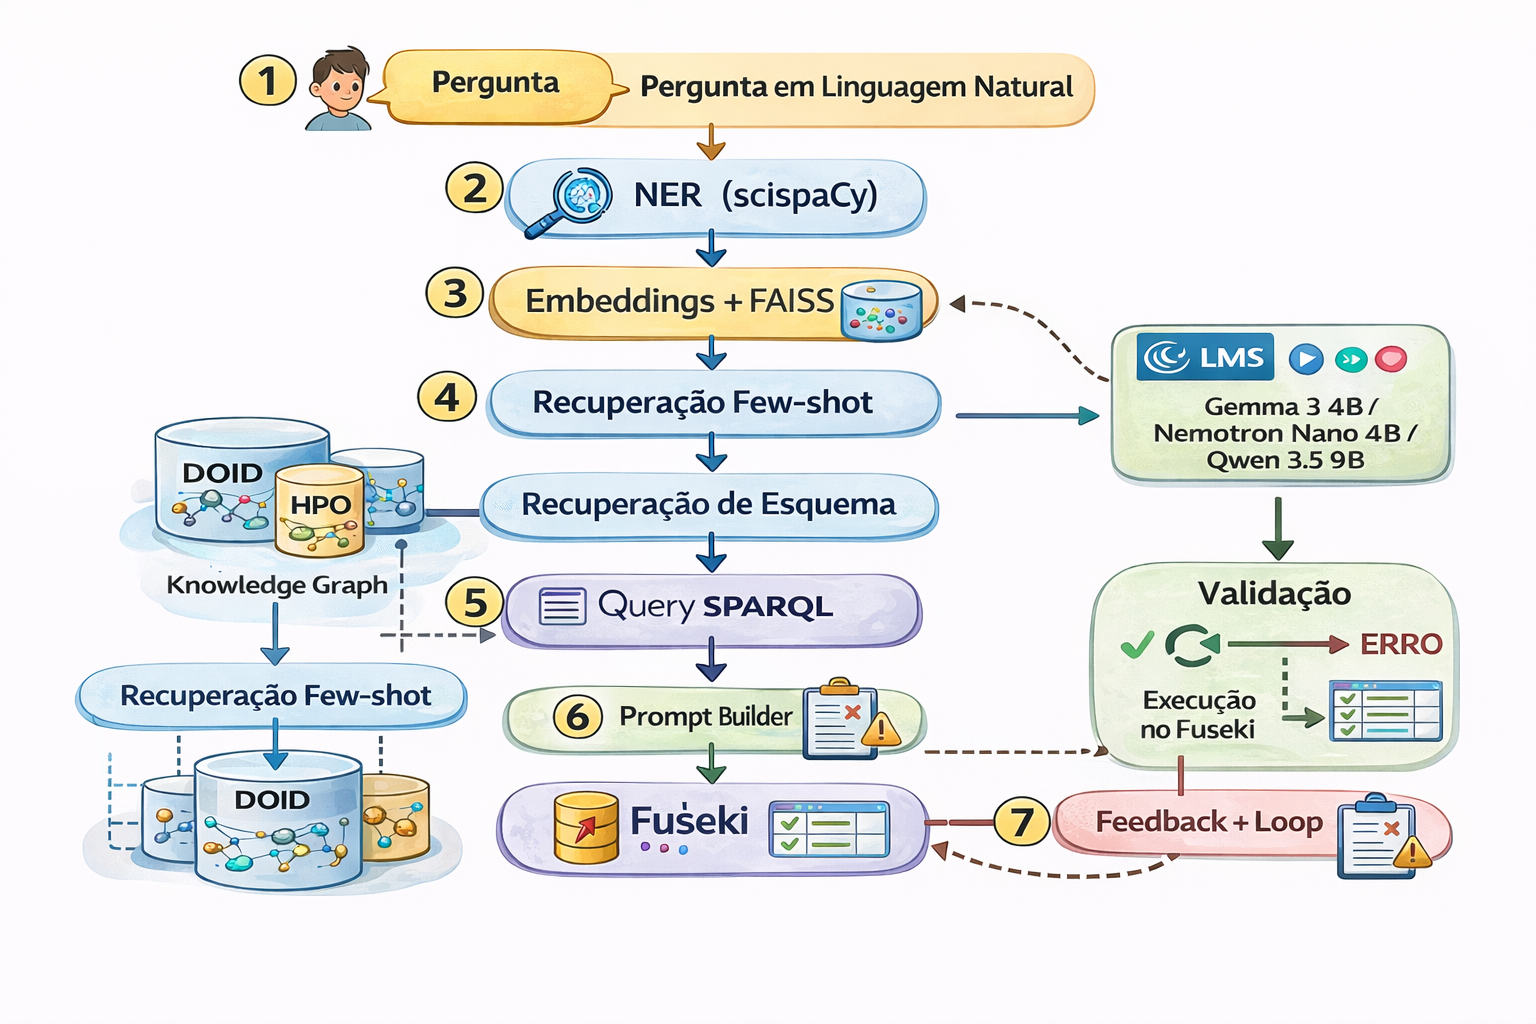
\includegraphics[width=0.55\textwidth]{arquitetura.png}
\caption{Arquitetura do pipeline BioSPARQL-NL.}
\label{fig:arquitetura}
\end{figure}

Os est\'{a}gios s\~{a}o: (1) a pergunta do usu\'{a}rio \'{e} processada por \textbf{scispaCy} para extra\c{c}\~{a}o de entidades nomeadas biom\'{e}dicas (NER); (2) embeddings da pergunta s\~{a}o usados para \textbf{recupera\c{c}\~{a}o FAISS} dos exemplos mais similares do \textit{gold standard}; (3) o \textbf{esquema ontol\'{o}gico} relevante \'{e} recuperado com base nas entidades identificadas; (4) um \textit{prompt} composto por exemplos \textit{few-shot}, esquema e pergunta \'{e} enviado ao \textbf{LLM} (Gemma 3 \cite{gemma2025}, Nemotron Nano \cite{nemotron2024} ou Qwen 3.5 \cite{qwen2025}, servidos localmente via LM Studio \cite{lmstudio2024}); (5) a consulta gerada passa por \textbf{valida\c{c}\~{a}o} sint\'{a}tica e de esquema; (6) se v\'{a}lida, \'{e} \textbf{executada} no Apache Jena Fuseki; caso contr\'{a}rio, o erro \'{e} adicionado ao \textit{prompt} e o ciclo se repete (m\'{a}ximo de 2 tentativas).

\subsection{Prepara\c{c}\~{a}o dos Dados}
\label{sec:dados}

O sistema opera sobre tr\^{e}s fontes de dados carregadas em um \textit{triplestore} Apache Jena Fuseki 6.0.0 \cite{jena2024fuseki} com backend TDB2:

\begin{itemize}
  \item \textbf{DOID} (\texttt{doid.owl}): Disease Ontology com mais de 12.000 classes de doen\c{c}as, carregada diretamente em formato OWL.
  \item \textbf{HPO} (\texttt{hp.owl}): Human Phenotype Ontology com mais de 16.000 termos fenot\'{i}picos, tamb\'{e}m em formato OWL.
  \item \textbf{HPOA} (\texttt{phenotype.hpoa}): anota\c{c}\~{o}es doen\c{c}a-fen\'{o}tipo distribu\'{i}das originalmente em formato TSV, convertidas para RDF/Turtle atrav\'{e}s de um script dedicado (\texttt{hpoa\_to\_rdf.py}).
\end{itemize}

Cada fonte \'{e} carregada em um \textit{named graph} separado no Fuseki, permitindo consultas espec\'{i}ficas por grafo ou consultas cruzadas (\textit{cross-graph}).

\subsection{Refer\^{e}ncias Cruzadas}
\label{sec:crossref}

Um desafio t\'{e}cnico relevante \'{e} a incompatibilidade de prefixos entre as fontes: a DOID utiliza o prefixo \texttt{MIM:} para refer\^{e}ncias ao OMIM, enquanto as anota\c{c}\~{o}es HPOA utilizam \texttt{OMIM:}. Para realizar jun\c{c}\~{o}es (\textit{joins}) entre doen\c{c}as e seus fen\'{o}tipos associados, o pipeline emprega constru\c{c}\~{o}es \texttt{BIND}/\texttt{REPLACE} no SPARQL para normalizar os identificadores em tempo de consulta, evitando duplica\c{c}\~{a}o de dados.

\subsection{Extra\c{c}\~{a}o de Esquemas}
\label{sec:schemas}

A extra\c{c}\~{a}o de esquemas \'{e} realizada por consultas SPARQL de introspec\c{c}\~{a}o executadas diretamente no Fuseki. Para cada \textit{named graph}, s\~{a}o extra\'{i}dos: (a) todas as classes instanciadas via \texttt{rdf:type}; (b) todas as propriedades utilizadas com seus dom\'{i}nios e contradom\'{i}nios efetivos; (c) contagens de triplas por propriedade. A agrega\c{c}\~{a}o \texttt{GROUP\_CONCAT} \'{e} utilizada para compactar listas de dom\'{i}nios/contradom\'{i}nios. O resultado \'{e} armazenado em \texttt{schemas.json} e disponibilizado ao pipeline como contexto para o \textit{prompt}.

\subsection{Pipeline NL$\rightarrow$SPARQL}
\label{sec:pipeline}

O pipeline completo opera da seguinte forma: dada uma pergunta em linguagem natural, o m\'{o}dulo de \textbf{liga\c{c}\~{a}o de entidades} utiliza scispaCy \cite{neumann2019scispacy} com o modelo \texttt{en\_core\_sci\_sm} para identificar men\c{c}\~{o}es a doen\c{c}as e fen\'{o}tipos. Em seguida, o m\'{o}dulo de \textbf{recupera\c{c}\~{a}o} utiliza Sentence-BERT \cite{reimers2019sbert} para gerar embeddings da pergunta e buscar os $k=3$ exemplos mais similares no \'{i}ndice FAISS \cite{johnson2021faiss} constru\'{i}do sobre o \textit{gold standard} de 52 quest\~{o}es curadas (13 f\'{a}ceis, 18 m\'{e}dias, 21 dif\'{i}ceis), validadas por concord\^{a}ncia inter-anotador (Cohen's $\kappa$) \cite{cohen1960kappa}.

O \textit{prompt} montado inclui: (1) instru\c{c}\~{o}es de sistema sobre a estrutura dos grafos; (2) esquema relevante em formato compacto; (3) exemplos \textit{few-shot} recuperados; e (4) a pergunta do usu\'{a}rio. O LLM, servido localmente via LM Studio \cite{lmstudio2024}, gera a consulta SPARQL. Tr\^{e}s modelos foram avaliados: Gemma 3 4B \cite{gemma2025}, Nemotron Nano 4B \cite{nemotron2024} e Qwen 3.5 9B \cite{qwen2025}.

O m\'{o}dulo de \textbf{valida\c{c}\~{a}o} verifica: (a) se a consulta \'{e} sintaticamente v\'{a}lida; (b) se todas as classes e propriedades referenciadas existem no esquema extra\'{i}do. Se a valida\c{c}\~{a}o falhar, a mensagem de erro \'{e} adicionada ao \textit{prompt} e uma nova tentativa \'{e} realizada, at\'{e} o m\'{a}ximo de 2 itera\c{c}\~{o}es.

\subsection{Interface XAI}
\label{sec:interface}

Para promover a Intelig\^{e}ncia Artificial Explic\'{a}vel (XAI), o sistema disponibiliza uma interface web constru\'{i}da com \textbf{React} no frontend e \textbf{FastAPI} no backend. A interface exibe: a consulta SPARQL gerada, as entidades reconhecidas pelo NER, o status de valida\c{c}\~{a}o (com detalhes de erros quando aplic\'{a}vel), a tabela de resultados retornados pelo Fuseki e uma decomposi\c{c}\~{a}o temporal (\textit{timing breakdown}) de cada est\'{a}gio do pipeline, permitindo ao usu\'{a}rio compreender e auditar todo o processo de tradu\c{c}\~{a}o.

%% ============================================================
\section{An\'{a}lise de Resultados e Conclus\~{a}o}
\label{sec:resultados}

Para avaliar o pipeline, foi definido um protocolo experimental com dois cen\'{a}rios (com e sem valida\c{c}\~{a}o por esquema) aplicados a tr\^{e}s modelos de linguagem distintos. A m\'{e}trica de \textbf{corre\c{c}\~{a}o} \'{e} definida como a propor\c{c}\~{a}o de quest\~{o}es cuja consulta gerada retornou ao menos o n\'{u}mero m\'{i}nimo de resultados esperado (\texttt{expected\_min\_results}), conforme especificado no \textit{gold standard}. A vers\~{a}o do DOID utilizada foi de abril/2026 (12.078 classes) e a do HPO de abril/2026 (908K triplas).

\subsection{Avalia\c{c}\~{a}o Multi-Modelo}
\label{sec:resultados_quant}

A avalia\c{c}\~{a}o foi realizada sobre o \textit{gold standard} de 30 quest\~{o}es (10 f\'{a}ceis, 10 m\'{e}dias, 10 dif\'{i}ceis), em dois cen\'{a}rios (com e sem valida\c{c}\~{a}o por esquema), utilizando tr\^{e}s modelos de linguagem dispon\'{i}veis localmente via LM Studio: \textbf{Gemma 3 4B} (Google, 4B), \textbf{Nemotron 3 Nano 4B} (NVIDIA, 4B) e \textbf{Qwen 3.5 9B} (Alibaba, 9B). A Tabela~\ref{tab:multimodelo} apresenta a compara\c{c}\~{a}o.

\begin{table}[H]
\centering
\caption{Compara\c{c}\~{a}o entre modelos (cen\'{a}rio com valida\c{c}\~{a}o por esquema).}
\label{tab:multimodelo}
\small
\begin{tabular}{lcccccc}
\toprule
\textbf{Modelo} & \textbf{Params} & \textbf{Sint\'{a}tica} & \textbf{Exec.} & \textbf{Corre\c{c}\~{a}o} & \textbf{Tempo} & \textbf{Tent.} \\
\midrule
Gemma 3        & 4B & 96,7\% & 70,0\% & 46,7\% & 4,3s  & 1,07 \\
Nemotron Nano  & 4B & 100\%  & 96,7\% & 80,0\% & 20,6s & 1,03 \\
Qwen 3.5       & 9B & 83,3\% & 66,7\% & 50,0\% & 63,4s & 2,23 \\
\bottomrule
\end{tabular}
\end{table}

A Tabela~\ref{tab:comvsem} compara o impacto da valida\c{c}\~{a}o por esquema na corre\c{c}\~{a}o de cada modelo.

\begin{table}[H]
\centering
\caption{Impacto da valida\c{c}\~{a}o por esquema na taxa de corre\c{c}\~{a}o.}
\label{tab:comvsem}
\small
\begin{tabular}{lcccc}
\toprule
\textbf{Modelo} & \textbf{Sem valid.} & \textbf{Com valid.} & \textbf{$\Delta$} & \textbf{Tent. m\'{e}d.} \\
\midrule
Gemma 3 4B    & 46,7\% & 46,7\% & 0,0pp  & 1,07 \\
Nemotron Nano & 86,7\% & 80,0\% & $-$6,7pp & 1,03 \\
Qwen 3.5 9B  & 0,0\%  & 50,0\% & +50,0pp & 2,23 \\
\bottomrule
\end{tabular}
\end{table}

O Qwen 3.5 apresenta o caso mais dr\'{a}stico: sem valida\c{c}\~{a}o, nenhuma de suas consultas retorna resultados corretos (0\% de corre\c{c}\~{a}o), mas com o la\c{c}o de autocorre\c{c}\~{a}o ativado (2,23 tentativas m\'{e}dias), atinge 50\%. Isso demonstra que a valida\c{c}\~{a}o por esquema \'{e} essencial para modelos que geram consultas inicialmente incorretas. Para o Nemotron, a valida\c{c}\~{a}o tem efeito ligeiramente negativo ($-$6,7pp), possivelmente por rejeitar consultas v\'{a}lidas que usam padr\~{o}es n\~{a}o capturados pelo esquema extra\'{i}do.

A Tabela~\ref{tab:dificuldade} detalha a taxa de corre\c{c}\~{a}o por n\'{i}vel de dificuldade para cada modelo.

\begin{table}[H]
\centering
\caption{Taxa de corre\c{c}\~{a}o por dificuldade e modelo (com valida\c{c}\~{a}o).}
\label{tab:dificuldade}
\begin{tabular}{lccc}
\toprule
\textbf{Modelo} & \textbf{F\'{a}cil (10)} & \textbf{M\'{e}dio (10)} & \textbf{Dif\'{i}cil (10)} \\
\midrule
Gemma 3 4B      & 60\% & 40\% & 40\% \\
Nemotron Nano   & 80\% & 80\% & 80\% \\
Qwen 3.5 9B    & 50\% & 30\% & 70\% \\
\bottomrule
\end{tabular}
\end{table}

%% Tabela detalhada por questao omitida por limitacao de espaco.
%% Resultados completos disponiveis em output/eval_*.json.

\subsection{Discuss\~{a}o}
\label{sec:discussao}

Os resultados revelam que a arquitetura e o treinamento do modelo s\~{a}o mais determinantes que o n\'{u}mero de par\^{a}metros. O Nemotron Nano (4B) alcan\c{c}ou 80\% de corre\c{c}\~{a}o, superando tanto o Gemma 3 (4B, 46,7\%) quanto o Qwen 3.5 (9B, 50\%). Surpreendentemente, o modelo maior (Qwen 3.5 9B) n\~{a}o superou significativamente o Gemma 3 4B em corre\c{c}\~{a}o geral, embora tenha apresentado desempenho superior em quest\~{o}es dif\'{i}ceis (70\% vs 40\%).

O Nemotron demonstrou vantagem em consultas \textit{cross-graph}, gerando corretamente jun\c{c}\~{o}es entre grafos com normaliza\c{c}\~{a}o MIM:/OMIM:. O Qwen 3.5 destacou-se em padr\~{o}es OPTIONAL + FILTER NOT BOUND e consultas hier\'{a}rquicas complexas. O Gemma 3 apresentou a menor corre\c{c}\~{a}o mas tamb\'{e}m o menor tempo de resposta (4,3s).

Todos os tr\^{e}s modelos falharam nas quest\~{o}es Q09 (xrefs com filtro OMIM espec\'{i}fico), Q14 (xref + fen\'{o}tipos em 3 grafos), Q16 (xrefs OMIM + ORPHA simult\^{a}neos) e Q30 (xrefs Orphanet como URLs). Esses padr\~{o}es envolvem conven\c{c}\~{o}es idiossincr\'{a}ticas do DOID que LLMs gen\'{e}ricos n\~{a}o possuem.

O Qwen 3.5 apresentou a maior taxa de retentativas (2,23 m\'{e}dia): sem valida\c{c}\~{a}o, 0\% de corre\c{c}\~{a}o; com autocorre\c{c}\~{a}o, 50\% --- demonstrando o valor pr\'{a}tico do mecanismo de retry via valida\c{c}\~{a}o de esquema.

O \textit{trade-off} tempo/qualidade \'{e} not\'{a}vel: Gemma 3 (4,3s) \'{e} 5x mais r\'{a}pido que Nemotron (20,6s) e 15x mais r\'{a}pido que Qwen 3.5 (63,4s). Para aplica\c{c}\~{o}es interativas, recomenda-se o Nemotron como melhor equil\'{i}brio entre qualidade e velocidade.

Comparando com trabalhos relacionados, o SPARQL-LLM \cite{emonet2024sparqlllm} tamb\'{e}m emprega RAG com valida\c{c}\~{a}o e autocorre\c{c}\~{a}o, mas foca em federa\c{c}\~{a}o multi-endpoint sobre KGs do SIB e n\~{a}o reporta taxas de corre\c{c}\~{a}o diretamente compar\'{a}veis. O KG-RAG \cite{soman2024kgrag} n\~{a}o gera SPARQL execut\'{a}vel, impossibilitando compara\c{c}\~{a}o direta. O BioSPARQL-NL se diferencia por ser o primeiro sistema espec\'{i}fico para jun\c{c}\~{o}es \textit{cross-graph} entre DOID, HPO e HPOA, operando inteiramente com modelos locais compactos (4B--9B) e gerando consultas SPARQL execut\'{a}veis e audit\'{a}veis, alinhado com princ\'{i}pios de IA explic\'{a}vel \cite{prenosil2025neurosymbolic}.

\subsection{Compara\c{c}\~{a}o Multi-Modelo (52 Quest\~{o}es)}
\label{sec:zeroshot}

Avaliamos sete modelos sobre as 52 quest\~{o}es (Tabela~\ref{tab:zeroshot}), do GPT-2 estilo ao Claude Sonnet como \textit{upper bound} comercial.

\begin{table}[H]
\centering
\caption{Compara\c{c}\~{a}o de sete modelos sobre 52 quest\~{o}es (cen\'{a}rio com valida\c{c}\~{a}o).}
\label{tab:zeroshot}
\scriptsize
\begin{tabular}{lccccc}
\toprule
\textbf{Modelo} & \textbf{Overall} & \textbf{F\'{a}cil} & \textbf{M\'{e}dio} & \textbf{Dif\'{i}cil} & \textbf{Sint.} \\
\midrule
BioGPT 1.5B$^*$        &  0,0\% &  0\% &  0\% &  0\% &  0,0\% \\
BioMedLM 2.7B$^*$      &  0,0\% &  0\% &  0\% &  0\% &  0,0\% \\
Gemma 3 4B             & 46,2\% & 38\% & 56\% & 43\% & 75,0\% \\
OpenBioLLM-8B          & 57,7\% & 77\% & 56\% & 48\% & 61,5\% \\
Llama3-Med42-8B        & 67,3\% & 85\% & 61\% & 62\% & 90,4\% \\
Qwen3-VL-8B            & 78,8\% & 77\% & 83\% & 76\% & 98,1\% \\
\textbf{Claude Sonnet} & \textbf{82,7\%} & \textbf{100\%} & \textbf{89\%} & \textbf{67\%} & \textbf{100,0\%} \\
\bottomrule
\multicolumn{6}{l}{$^*$GPT-2 style, sem \textit{instruction-following}.}
\end{tabular}
\end{table}

Modelos sem \textit{instruction-following} atingem 0\%; o Qwen3-VL-8B (78,8\%) aproxima-se do Claude Sonnet em 3,9pp; o Llama3-Med42-8B (67,3\%) supera o Gemma 3 4B em 21,1pp pelo ajuste biom\'{e}dico.


\subsection{Estudo de Abla\c{c}\~{a}o}
\label{sec:ablacao}

A Tabela~\ref{tab:ablacao} apresenta o estudo de abla\c{c}\~{a}o sobre o Gemma 3 4B (30 quest\~{o}es): \textit{few-shot} e esquema contribuem +3,3pp cada; NER reduz a corre\c{c}\~{a}o em 13,3pp (liga\c{c}\~{a}o de entidades introduz ru\'{i}do neste modelo); e zero-shot (66,7\%) supera o pipeline completo (50,0\%), indicando efeito aditivo negativo dos componentes para LLMs compactos.

\begin{table}[H]
\centering
\caption{Estudo de abla\c{c}\~{a}o --- Gemma 3 4B (30 quest\~{o}es).}
\label{tab:ablacao}
\small
\begin{tabular}{lccc}
\toprule
\textbf{Configura\c{c}\~{a}o} & \textbf{Sint.} & \textbf{Corre\c{c}\~{a}o} & \textbf{$\Delta$ vs Full} \\
\midrule
Full Pipeline         & 90,0\% & 50,0\% & ---        \\
$-$ NER               & 90,0\% & 63,3\% & +13,3pp    \\
$-$ Few-shot          & 90,0\% & 46,7\% & $-$3,3pp   \\
$-$ Schema            & 76,7\% & 46,7\% & $-$3,3pp   \\
$-$ Valida\c{c}\~{a}o & 66,7\% & 50,0\% & 0,0pp      \\
Zero-shot             & 86,7\% & 66,7\% & +16,7pp    \\
\bottomrule
\end{tabular}
\end{table}

\subsection{Limita\c{c}\~{o}es}
\label{sec:limitacoes}

As principais limita\c{c}\~{o}es identificadas s\~{a}o:

(1) \textbf{Hardware como gargalo}: apenas modelos $\leq$4B operam na GPU (8GB VRAM) sem degrada\c{c}\~{a}o. O Qwen 3.5 9B, com \textit{offload} parcial para CPU, foi 15$\times$ mais lento que o Gemma 3 4B (63,4s vs 4,3s) e avaliado apenas nas 30 quest\~{o}es prim\'{a}rias.
(2) \textbf{Conven\c{c}\~{o}es idiossincr\'{a}ticas}: a incompatibilidade MIM:/OMIM: entre DOID e HPOA contribui para parte das 9 falhas irredut\'{i}veis (mesmo com Claude Sonnet).
(3) \textbf{Falhas silenciosas}: 86\% das falhas locais s\~{a}o consultas sint\'{a}ticas v\'{a}lidas com zero resultados --- sem sinal de erro ao usu\'{a}rio.
(4) \textbf{Variabilidade estoc\'{a}stica}: o Gemma 3 4B variou $\pm$3 quest\~{o}es entre execu\c{c}\~{o}es id\^{e}nticas (\texttt{temperature=0.1}).
(5) \textbf{Generaliza\c{c}\~{a}o limitada}: sobre o QALD-9+ \cite{qaldnineplus} (DBpedia, 30q), o pipeline executou SPARQL em 80\% das quest\~{o}es, mas atingiu F1=0,106 sem adapta\c{c}\~{a}o de dom\'{i}nio.

\subsection{Conclus\~{a}o}
\label{sec:conclusao}

Este trabalho apresentou o BioSPARQL-NL, o primeiro pipeline NL$\rightarrow$SPARQL para DOID, HPO e HPOA. A avalia\c{c}\~{a}o com sete modelos produziu cinco achados:

(a) \textbf{Valida\c{c}\~{a}o \'{e} essencial}: sem valida\c{c}\~{a}o por esquema, Gemma 3 4B cai de 46,2\% para 25,0\% e Claude Sonnet de 82,7\% para 46,2\% --- o la\c{c}o de autocorre\c{c}\~{a}o \'{e} o componente mais cr\'{i}tico.
(b) \textbf{Arquitetura supera tamanho}: Nemotron Nano 4B atingiu 80,0\% nas 30 quest\~{o}es prim\'{a}rias, superando Qwen 3.5 9B (50,0\%).
(c) \textbf{Gap local--comercial reduzido}: Qwen3-VL-8B (78,8\%) fica a apenas 3,9pp do Claude Sonnet (82,7\%); modelos biom\'{e}dicos instruct (Llama3-Med42: 67,3\%) superam modelos gerais de igual porte, mas GPT-2 style sem \textit{instruction-following} atingem 0\%.
(d) \textbf{Erros irredut\'{i}veis}: 9 quest\~{o}es (17,3\%) falharam mesmo com Claude Sonnet (MIM:/OMIM: e complexidade combinat\'{o}ria).
(e) \textbf{Transferibilidade parcial}: no QALD-9+ \cite{qaldnineplus} (DBpedia, 30q), execu\c{c}\~{a}o em 80\% mas F1=0,106 --- adapta\c{c}\~{a}o de dom\'{i}nio \'{e} necess\'{a}ria para corre\c{c}\~{a}o sem\^{a}ntica.

Trabalhos futuros: \textit{fine-tuning} biom\'{e}dico; valida\c{c}\~{a}o sem\^{a}ntica p\'{o}s-execu\c{c}\~{a}o; avalia\c{c}\~{a}o com usu\'{a}rios reais; expans\~{a}o para 100+ quest\~{o}es.

%% ============================================================

\bibliographystyle{sbc}
\bibliography{biosparql-nl}

\end{document}
